\begin{frame}{Results (3): Pattern of map changes}

\begin{figure}[tb]
    \begin{center}
        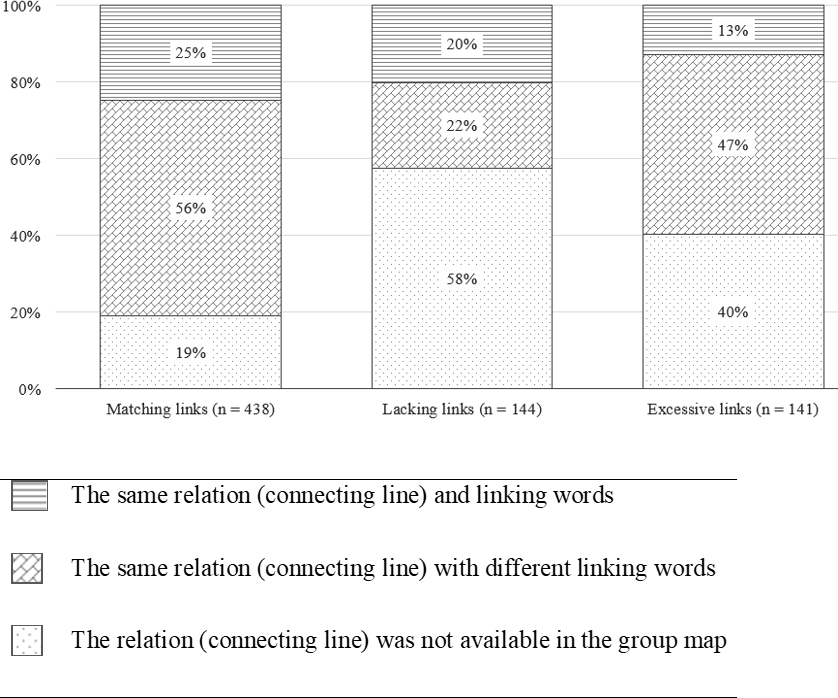
\includegraphics[width=50mm]{images/dist_match_links.pdf}
    \end{center}
    \caption{Proportions of the individual propositions taken from the system,with  the  matching,  lacking,  and  excessive  links,  compared  to  the  group propositions}
    \label{a1::map_sample_1}
\end{figure}

\end{frame}
% \begin{frame}{Results (3): Pattern of map changes based on the visualization}

%    \begin{columns}
%        \begin{column}{0.5\textwidth}
%            \begin{center}
%                \begin{figure}[tb]
%                \includegraphics[width=55mm]{/images/rqa_map_patterns_b.pdf}
                    %\caption{Scatter plot of group prior knowledge similarity and normalized gain from individual to collaborative map}
                    %\label{prior_gain}
%                \end{figure}
%            \end{center}
%        \end{column}
%        \begin{column}{0.5\textwidth}  %%<--- here
%            \begin{center}
%                \begin{figure}[tb]
%                \includegraphics[width=50mm]{/images/rqa_map_patterns_a.pdf}
                    %\caption{Scatter plot of group comprehension level and normalized gain from 
                    %individual to collaborative map}
                    %\label{comprehension_gain}
%               \end{figure}
%            \end{center}
%        \end{column}
%    \end{columns} 
    
    
    %\begin{figure}[tb]
    %\begin{center}
    %    \includegraphics[width=50mm]{images/rqa_map_patterns_a.pdf}
    %\end{center}
    
    %\label{a1::map_sample_1}
    %\end{figure}
% \end{frame}


%\begin{frame}{Results (3): Pattern of map changes based on the visualization}
%    \begin{figure}[tb]
%    \begin{center}
%        \includegraphics[width=80mm]{images/rqa_map_patterns_b.pdf}
%    \end{center}
%    \caption{The  number  of  propositions  from  the  individual  to  the  groupmaps were categorized by the link types in the KB-map, the similarity be-tween the KB-map proposition and the group-map proposition, and the levelof group proposition correctness}
%    \label{a1::map_sample_2}
%\end{figure}
%\begin{block}{Finding \#3}
%\begin{itemize}
%    \item <+->Students \textcolor{teal}{thought deeply} about the propositions and found out the correct representation. 
%    \item <+-> Besides, Pearson’s correlation analysis depicted that there was a \textcolor{teal}{moderate positive correlation} between the score differences and the number of excessive links presented in the KB analyzer (R(21) = 0.58, p < .01).
%\end{itemize}
%\end{block}

%\end{frame}

\begin{frame}{1) Similarity of prior knowledge: formulae}
    \begin{itemize}
        \item A graph \textit{G} = (\textit{V}, \textit{E}) is a finite set $V$ 
        of $n$ nodes and a set \textit{E} of edges, where \textit{E} is a 
        subset of $V \times V$.
        \item Given two undirected and labeled graphs, $A = (V, E_A)$ and 
        $B = (V, E_B)$, with common node set $V$, $S(A, B)$ is the similarity 
        between $A$ and $B$ as measured by $S$. 
        \item $SE_{AB}$ consists of shared links between $E_A$ and $E_B$ 
        while $UE_{AB}$ contains a set of unshared links created by 
        only one of the group members.
    \end{itemize}
\end{frame}

\begin{frame}{1) Similarity of prior knowledge: formulae (cont'd)}
    \begin{equation}
      SE_{AB} = E_A \cap E_B \label{eq:1}
    \end{equation}
    
    \begin{equation}
      UE_{AB} = E_A \ominus E_B \label{eq:2}
    \end{equation}
    
    \begin{equation}
      S(A, B) = \frac{|SE_{AB}|}{{|SE_{AB}| + \frac{|UE_{AB}|}{2}}} \label{eq:3}
    \end{equation}
    
    $S(A, B)$ represents \textcolor{blue}{the similarity score of two initial maps}
\end{frame}

\begin{frame}{1) Similarity of prior knowledge: linking words similarity}
    \begin{itemize}
        \item Pre-processing techniques: text normalization 
              (e.g., transforming to lower case, removing punctuation, stemming) 
              and stop-word removal
        \item Applying \textcolor{blue}{Term Frequency - Inverse Document Frequency (TF-IDF) cosine similarity} formula to get the linking-word similarity
        \item It falls into three following categories: 
        \begin{itemize}
            \item \textbf{no similarity} if the score is 0; 
            \item \textbf{moderately low similarity} if the score lies between 0--.509;
            \item \textbf{moderately high similarity} if greater than .509.
        \end{itemize} 
        \item This categorization is based on the first and third quartiles 
        of the similarity score distribution ($M = .27, SD = .34, Q1 = 0, Q3 = .509$).
    \end{itemize}
\end{frame}

\begin{frame}{2): Comprehension of partner's map components}

\begin{itemize}
    \item <+-> A graph $G_A = (V, E_A)$ is a finite set $V$ of $n$ nodes and a set $E$ of edges built by student $A$. 
    \item <+-> A graph $R_A = (V, E_{RA})$ is a graph re-constructed by student $A$'s partner. 
    \item <+-> Let $E_{MA}$ be the set of $A$'s first map links that are connected to the same nodes by the partner in the second map, while $E_{NA}$ consists of the links that are joined to different nodes.
    \item <+-> \begin{equation}
            E_{MA} = E_{RA} \cap E_A 
    \end{equation}
    \item <+-> \begin{equation}
            E_{NA} = E_{RA} \ominus E_A
    \end{equation}
    \\
    \item <+-> The element of $E_{MA}$ is called a reconstructed link, while $E_{NA}$ consists of non-reconstructed links.
\end{itemize}

\end{frame}

\begin{frame}{2): Comprehension of partner's map components (cont'd)}

Given two undirected and labeled re-constructional graphs $R_A$ and $R_B$ with common node set $V$, 
$C(A, B)$ is the comprehension value between student $A$ and $B$, as a pair in a group, defined as: 

\begin{equation}
  C(A, B) = \frac{|E_{MA} + E_{MB}|}{|E_{MA} + E_{MB}| + \frac{|E_{NA} + E_{NB}|}{2}} 
  \label{eq:6}
\end{equation}

\end{frame}

\begin{frame}{3)Similarity of individual and group map linking words}

\begin{itemize}
    \item Applying some pre-processing techniques and \textcolor{blue}{Term Frequency - Inverse Document Frequency (TF-IDF) cosine similarity} formula to get the linking-word similarity
    \item It falls into three following categories: 
    {\small \begin{itemize}
        \item \textbf{follow initial}: the group of linking words that are similar with at least one of the individual linking words (similarity value of equal to or more than .99);
        \item \textbf{modify initial}: the group of linking words that are modified from one of the individual linking words (similarity value above .366 and below .99);
        \item \textbf{new}: the group of linking words that are not similar to any of the individual linking words (similarity value of below .366).
    \end{itemize}} 
    \item This categorization is based on the first and third quartiles 
    of the similarity score distribution ($M = .68, SD = .37, Q1 = .366, Q3 = 1$).
\end{itemize}

\end{frame}

\begin{frame}{Data measurements (4): Map score change}

To measure the change of map score from the individual to the collaborative phase, this 
study adopts the normalized change formula proposed by Marx and Cummings 

%\cite{Marx2007NormalizedChange}.

\begin{equation}
 c =
    \begin{cases}
        \frac{gms - ais}{100 - ais} & \text{if $gms$ > $ais$}\\
        $drop$ & \text{if $gms$ = $ais$ = 100 or 0} \\
        0 & \text{if $gms$ = $ais$}\\
        \frac{gms - ais}{ais} & \text{if $gms$ < $ais$}
    \end{cases}
    \label{eq:7}
\end{equation}
    
\end{frame}


\begin{frame}{Sample of map transformation: 1}
    \begin{figure}[tb]
    \begin{center}
        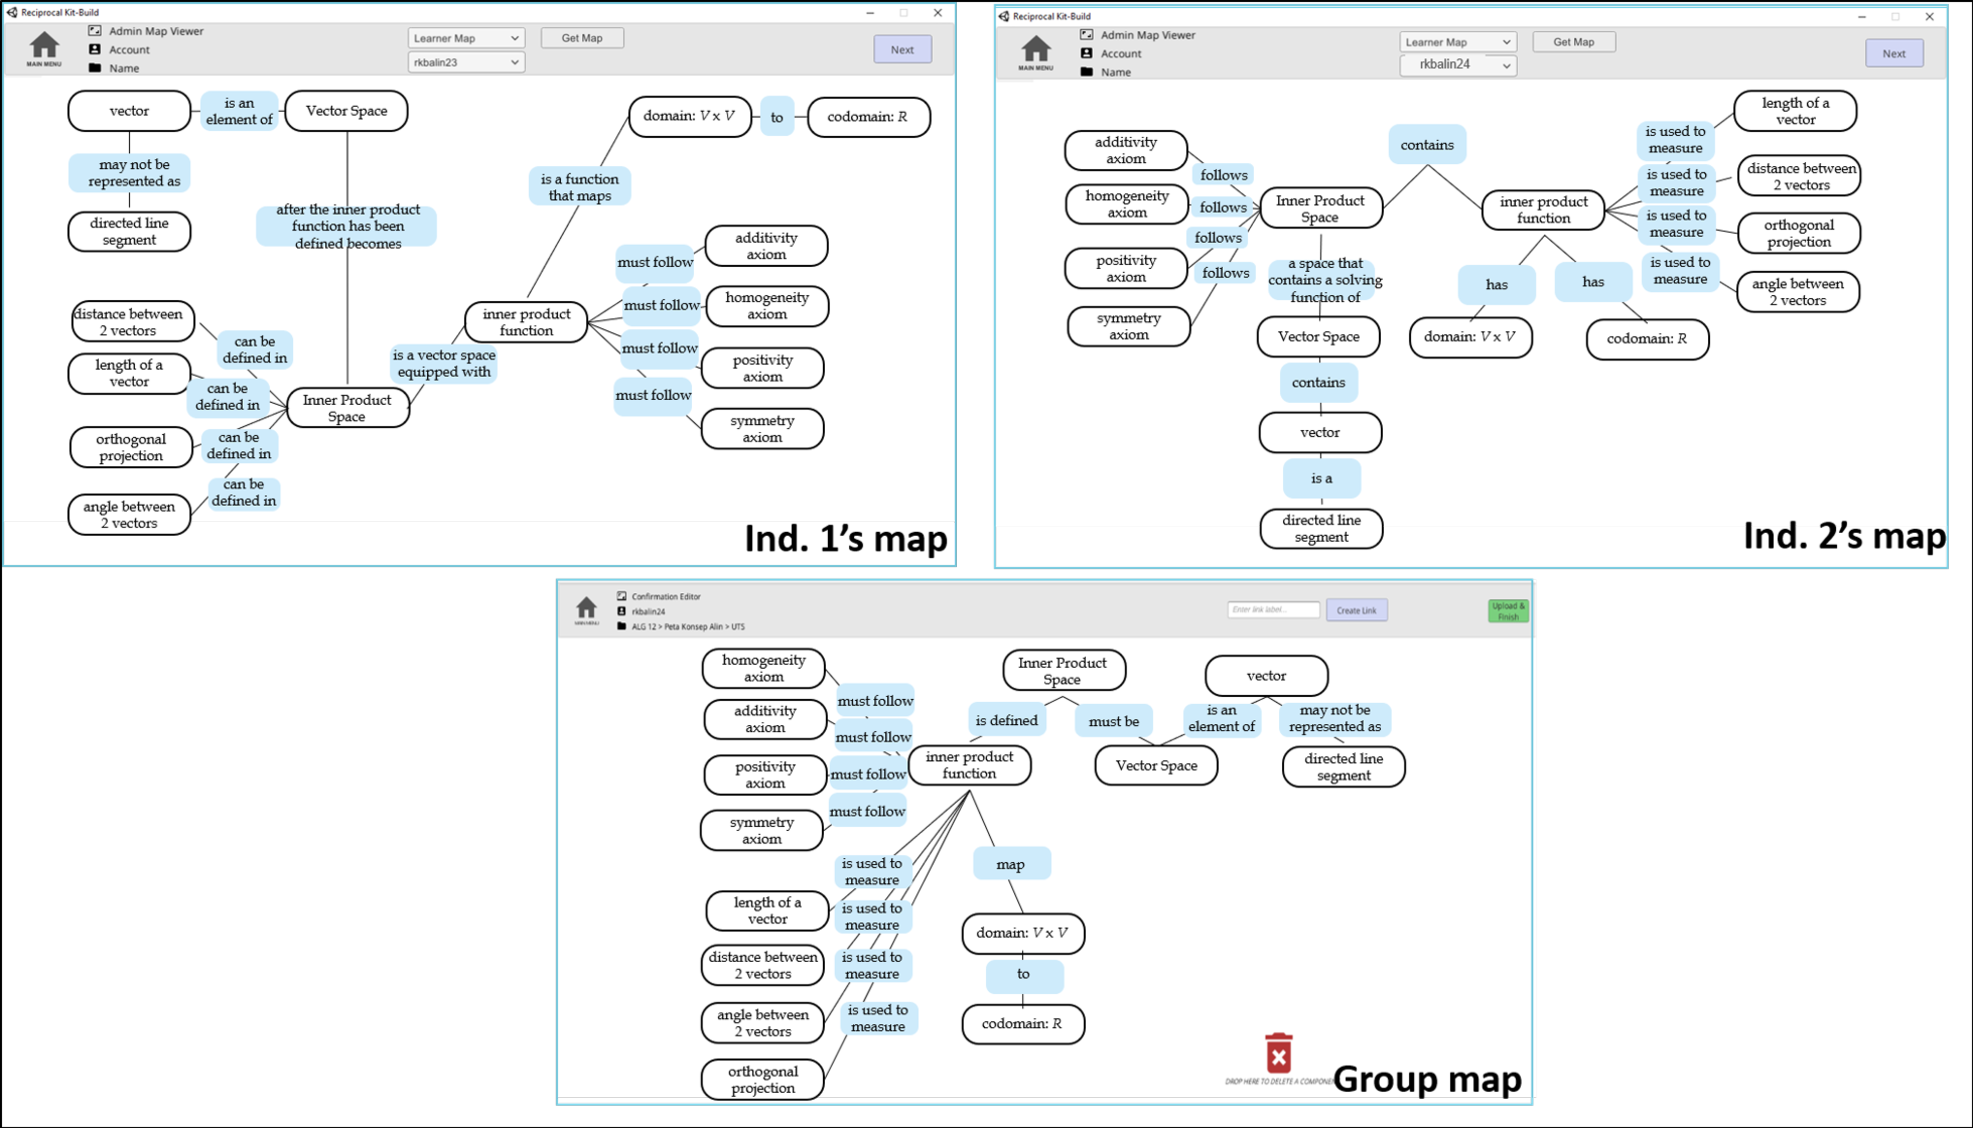
\includegraphics[width=100mm]{images/a1_dist_correctness.pdf}
    \end{center}
    \caption{Sample of individual maps and group map generated by group ALG12}
    \label{a1::map_sample}
\end{figure}
\end{frame}

\begin{frame}{Sample of map transformation: 2}
    \begin{figure}[tb]
        \begin{center}
            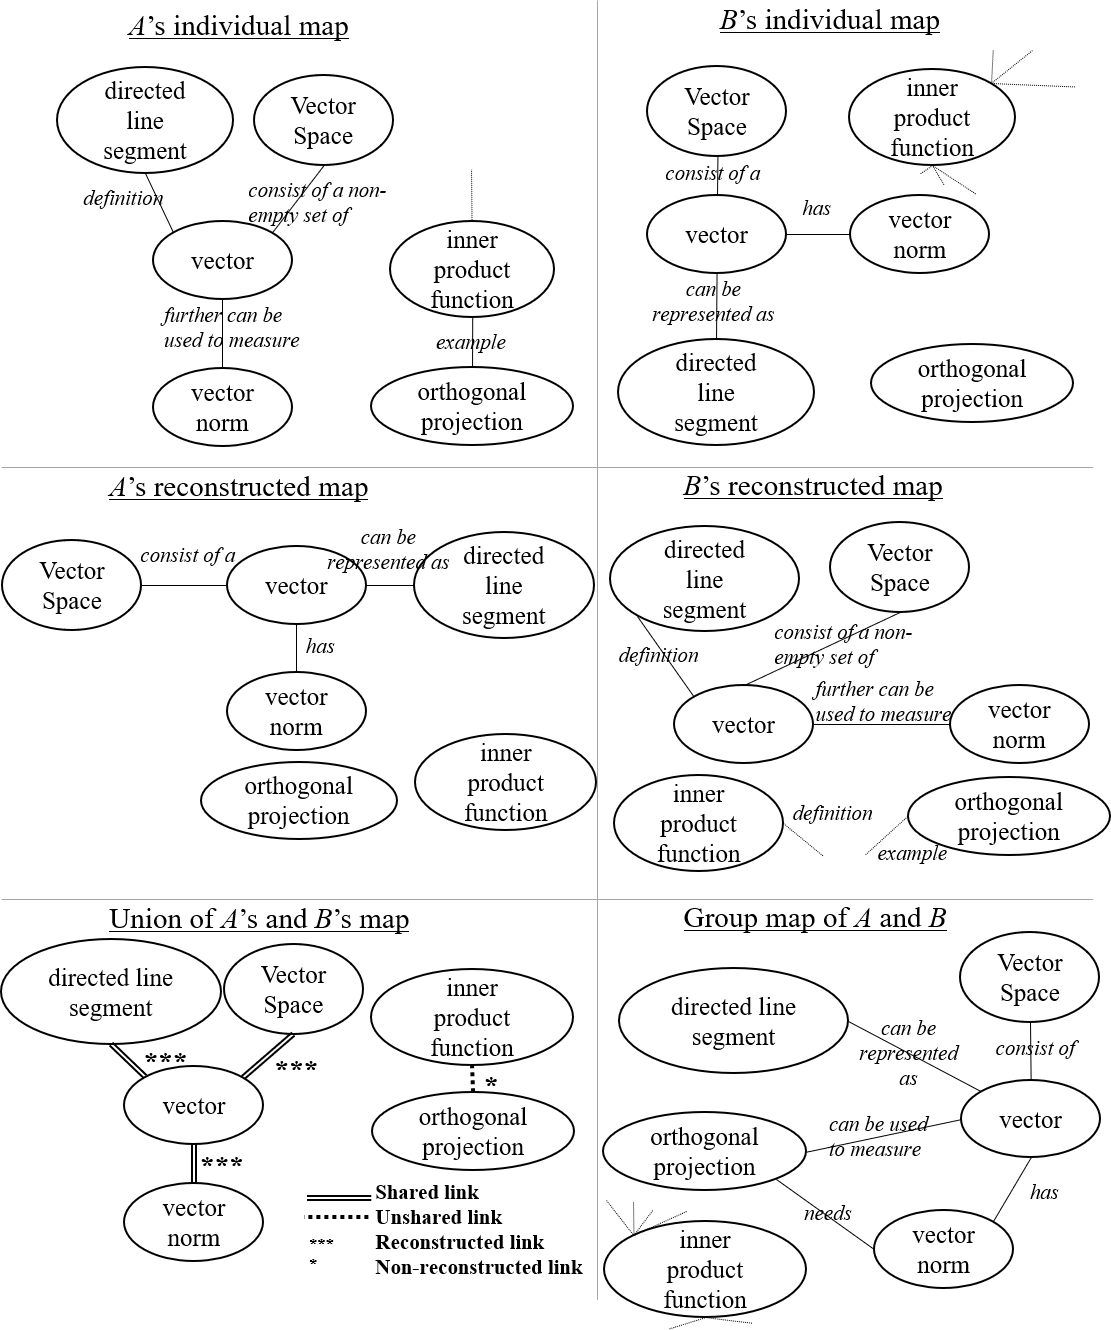
\includegraphics[width=50mm]{images/a3_sample_of_map.pdf}
        \end{center}
        \caption{Sample of individual maps of two students in a group, their reconstructed maps,
            the corresponding union map with the categorization of links, and the 
            newly transformed group map}
        \label{map_sample}
    \end{figure} 
\end{frame}

\begin{frame}{Acknowledgement}
    <div>Icons made by <a href="https://www.flaticon.com/authors/nikita-golubev" title="Nikita Golubev">Nikita Golubev</a> from <a href="https://www.flaticon.com/" title="Flaticon">www.flaticon.com</a></div>
    <div>Icons made by <a href="https://www.flaticon.com/authors/freepik" title="Freepik">Freepik</a> from <a href="https://www.flaticon.com/" title="Flaticon">www.flaticon.com</a></div>
    <div>Icons made by <a href="https://www.flaticon.com/authors/freepik" title="Freepik">Freepik</a> from <a href="https://www.flaticon.com/" title="Flaticon">www.flaticon.com</a></div>
\end{frame}

\begin{frame}{Thesis structure}
   \begin{figure}[tb]
       \begin{center}
           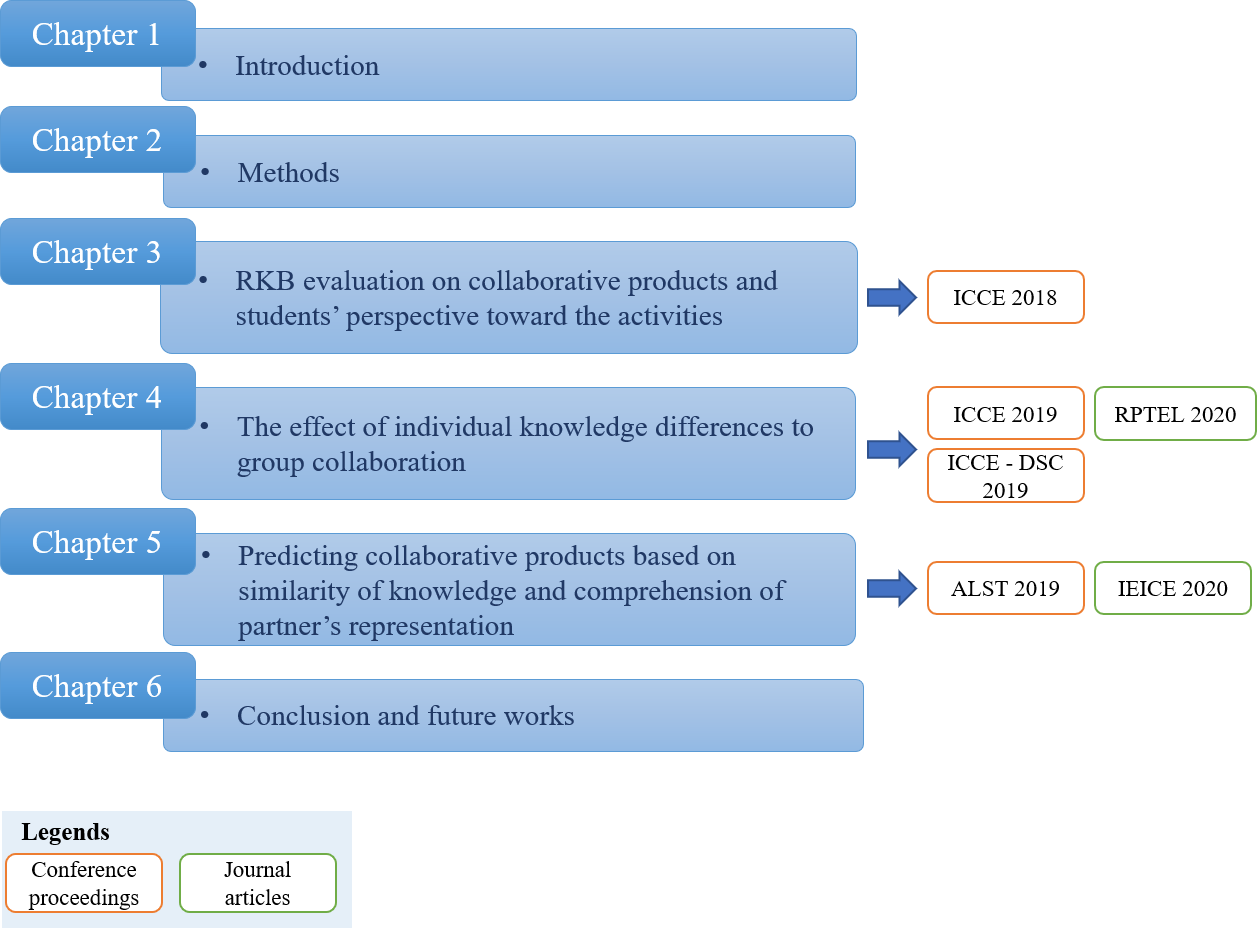
\includegraphics[width=95mm]{images/thesis_structures.pdf} 
       \end{center}
       \caption{Thesis structure and relevant publications}
       \label{thesis_struct}
   \end{figure}
\end{frame}

\begin{frame}[allowframebreaks]{Concept map evaluation}
   \begin{figure}[tb]
       \begin{center}
           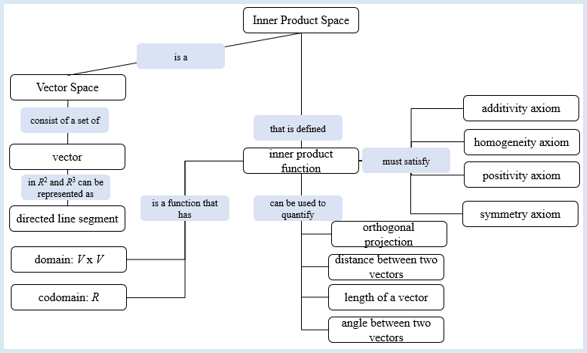
\includegraphics[width=95mm]{images/expert_map.png} 
       \end{center}
    %   \caption{Thesis structure and relevant publications}
    %   \label{thesis_struct}
   \end{figure}
   The experiment was conducted in a regular classroom, with one teacher. 
Concept map evaluation was performed by the teacher, not the researcher. 
Before the experiment, the teacher had composed an expert map.
She then developed a grading rubric accordingly, based on the completeness of information in the student’s map and its accuracy. 
One type of information may be conveyed by different propositions, but variation were limited because the subject was Mathematics. 

\end{frame}